\documentclass[twoside,doctor,numberorder]{zjuthesis}
%==============================================================
%==============================================================

%自己需要增加什么 package 或修改什么设置的话,都放在这里吧。
%\usepackage{xxxx}

%==============================================================
%==============================================================
\begin{document}
%==============================================================
%==============================================================
%这部分是论文封面、题名页需要的信息,请根据《研究生学位论文编写规则》自行修改

  % {论文分类号}{论文密级}
  \zjutype{C936}{}
  %论文题目:{中文}{英文}
  \zjutitle{基于成本的钉耙强度与应用——东方视角分析}%
           {Cost Based Rake Strength and Application: An Oriental View}
  %作者:{姓名}{学号}
  \zjuauthor{猪八戒}{10320022}
  %指导教师:{导师}{合作导师}
  \zjumentor{唐三藏}{}
  %个人信息:{研究方向}{专业名称}{学院}
  \zjuinfo{法器工程}{祭坛管理}{大雷音寺管理研究院}
  %日期:{提交日期}{答辩日期中文}{答辩日期英文}
  \zjudate{二〇〇八年九月}{二〇〇八年十二月}{December 2008}
  %论文评阅人:{评阅人中文姓名}{评阅人英文姓名}
  %格式:姓名$\backslash$职称$\backslash$单位
  \zjureviewerone{}{}
  \zjureviewerone{}{}
  \zjureviewerone{}{}
  \zjureviewerone{}{}
  \zjureviewerone{}{}
  %答辩委员会:{委员中文姓名}{委员英文姓名}
  %格式:姓名$\backslash$职称$\backslash$单位
  \zjucommitteemain{弥勒$\backslash$佛$\backslash$大雷音寺}%
                   {Maitreya$\backslash$Buddha$\backslash$Thunder Monastery}
  \zjucommitteeone{观音$\backslash$菩萨$\backslash$补陀落迦山}%
                  {Avalokiteśvara$\backslash$Bodhisattva$\backslash$Potalaka}
  \zjucommitteetwo{地藏王$\backslash$菩萨$\backslash$九华山}%
                  {Ksitigarbha$\backslash$Bodhisattva$\backslash$Jiuhua Mountain}
  \zjucommitteethree{阿氏多$\backslash$罗汉$\backslash$鹫峰山}%
                    {Ajita$\backslash$Arhat$\backslash$Jiufeng Mountain}
  \zjucommitteefour{广成子$\backslash$仙人$\backslash$崆峒山}%
                   {GuangCheng-Zi$\backslash$Immortal$\backslash$Kongtong Mountain}
  \zjucommitteefive{}{}

%==============================================================
% 这部分除了“取舍”外,不需要自己修改,必要信息都已在上面设置。

  %封面
  %%============================================================
%% 中文封面

\thispagestyle{empty}

\vspace{5mm}

\begin{center}
   
\includegraphics[width=108mm]{images/zjdx}
\end{center}

\centerline{\songti\erhao\textbf{本科生毕业论文(设计)}}

\vspace{4mm}

\begin{center}
  
\includegraphics[width=35mm]{images/standxb}
\end{center}

\vspace{25mm}

\begin{tabbing}
\hspace{16mm}\songti\sanhao\bfseries 题目: \= \hspace{0mm} \= \parbox[t]{98mm}{%
  \begin{picture}(0,0)(0,0)
  \setlength{\unitlength}{1cm}
    \put(0,-0.2){\line(1,0){9.8}}
  \end{picture}%
\linespread{1.1}\bfseries\Large\zjutitlec} \\[3mm]
\end{tabbing}

\vspace{4mm}

\begin{tabbing}
    \hspace{30mm} \songti\sihao 姓 \hspace{-2.7mm} \= \songti\sihao 名与学号: \= \underline{\makebox[6cm]{\sihao\zjuauthornamec\hspace{3mm}\zjuauthorid}} \\[2mm]
              \> \songti\sihao 指导教师: \> \underline{\makebox[6cm]{\sihao\zjumentorc}} \\[2mm]
              \hspace{30mm} \songti\sihao 年 \hspace{-2.7mm} \= \songti\sihao 级与专业: \= \underline{\makebox[6cm]{\sihao\zjugrade\hspace{3mm}\zjumajor}} \\[2mm]
              \> \songti\sihao 所在学院: \> \underline{\makebox[6cm]{\sihao\zjucollegec}}
\end{tabbing}


%%============================================================
% empty page for two-page print
\ifthenelse{\equal{\zjuside}{T}}{%
  \newpage\mbox{}%
  \thispagestyle{empty}}{}

%%============================================================
%% English Cover
\newpage
\thispagestyle{empty}

\vspace{5mm}

\begin{center}
    \songti\xiaoyi A Dissertation Submitted to Zhejiang University for the Degree of Bachelor of Engineering
\end{center}

\vspace{4mm}

\begin{center}
  
\includegraphics[width=35mm]{images/standxb}
\end{center}

\vspace{25mm}

\begin{tabbing}
\hspace{8mm}\songti\sanhao\bfseries TITLE: \= \hspace{0mm} \= \parbox[t]{124mm}{%
  \begin{picture}(0,0)(0,0)
  \setlength{\unitlength}{1cm}
    \put(0,-0.2){\line(1,0){12.4}}
  \end{picture}%
\linespread{1.1}\bfseries\Large\zjutitlee} \\[3mm]
\end{tabbing}

\vspace{4mm}

\begin{tabbing}
    \hspace{18mm} \= \sanhao Author:\hspace{19mm} \= \underline{\makebox[8cm]{\sanhao\zjuauthornamee\hspace{3mm}\zjuauthorid}} \\[2mm]
                  \> \sanhao Supervisor: \> \underline{\makebox[8cm]{\sanhao\zjumentore}} \\[2mm]
                  \> \sanhao Subject: \> \underline{\makebox[8cm]{\sanhao\zjusubject}} \\[2mm]
                  \> \sanhao College: \> \underline{\makebox[8cm]{\sanhao\zjucollegee}} \\[2mm]
                  \> \sanhao Submitted Date: \> \underline{\makebox[8cm]{\sanhao\zjusubmitteddatee}}
\end{tabbing}

%%============================================================
% empty page for two-page print
\ifthenelse{\equal{\zjuside}{T}}{%
  \newpage\mbox{}%
  \thispagestyle{empty}}{}

  %中文题名页
  %%% 中文提名页

\newpage
\thispagestyle{empty}

\vspace{5mm}

\begin{center}
\parbox{0.75\linewidth}{%
  \begin{picture}(0,0)(0,0)
  \setlength{\unitlength}{1cm}
    \put(0,-0.2){\line(1,0){11.3}}
    \put(0,-1.1){\line(1,0){11.3}}
  \end{picture}%
  \linespread{1.1}\xiaoer\bfseries\zjutitlec}
\end{center}

\vspace{5mm}

\begin{center}
  
\includegraphics[width=21mm]{images/standxb.pdf}
\end{center}

\vspace{3mm}

\begin{tabbing}
\hspace{30mm} \= \songti\xiaosan\bfseries 论文作者签名: \= \underline{\makebox[5cm]{}} \\[8mm]
              \> \songti\xiaosan\bfseries 指导教师签名: \> \underline{\makebox[5cm]{}}
\end{tabbing}

\vspace{8mm}

\begin{tabbing}
\hspace{10mm} \songti\sihao 论文 \hspace{-2mm} \= \songti\sihao 评阅人 1: \= \underline{\makebox[9cm]{\sihao\zjurevieweronec}} \\
              \> \songti\sihao 评阅人 2: \> \underline{\makebox[9cm]{\sihao\zjureviewertwoc}} \\
              \> \songti\sihao 评阅人 3: \> \underline{\makebox[9cm]{\sihao\zjureviewerthreec}} \\
              \> \songti\sihao 评阅人 4: \> \underline{\makebox[9cm]{\sihao\zjureviewerfourc}} \\
              \> \songti\sihao 评阅人 5: \> \underline{\makebox[9cm]{\sihao\zjureviewerfivec}}
\end{tabbing}

\vspace{8mm}

\begin{tabbing}
\hspace{5mm}\songti\sihao 答辩委员 \hspace{-2.2mm} \= \songti\sihao 会主席: \= \underline{\makebox[9cm]{\sihao\zjucommitteemainc}} \\
          \>    \songti\sihao ~委员 1: \> \underline{\makebox[9cm]{\sihao\zjucommitteeonec}} \\
          \>    \songti\sihao ~委员 2: \> \underline{\makebox[9cm]{\sihao\zjucommitteetwoc}} \\
          \>    \songti\sihao ~委员 3: \> \underline{\makebox[9cm]{\sihao\zjucommitteethreec}} \\
          \>    \songti\sihao ~委员 4: \> \underline{\makebox[9cm]{\sihao\zjucommitteefourc}} \\
          \>    \songti\sihao ~委员 5: \> \underline{\makebox[9cm]{\sihao\zjucommitteefivec}}
\end{tabbing}

\vspace{8mm}

\begin{tabbing}
\hspace{34mm} \= \songti\sihao 答辩日期: \= \underline{\makebox[5cm]{\songti\sihao\zjudefencedatec}} \\
\end{tabbing}

\ifthenelse{\equal{\zjuside}{T}}{%
  \newpage\mbox{}%
  \thispagestyle{empty}}{}

  %英文题名页
  %%% 英文提名页

\newpage
\thispagestyle{empty}

\vspace{5mm}

\begin{center}
\parbox{0.75\linewidth}{%
  \begin{picture}(0,0)(0,0)
  \setlength{\unitlength}{1cm}
    \put(0,-0.2){\line(1,0){11.3}}
    \put(0,-1.1){\line(1,0){11.3}}
  \end{picture}%
  \linespread{1.4}\large\bfseries\zjutitlee}
\end{center}

\vspace{5mm}

\begin{center}
  
\includegraphics[width=21mm]{images/standxb.pdf}
\end{center}

\vspace{-6mm}

\begin{tabbing}
\hspace{20mm} \= \large\bfseries Supervisor's signature: \= \underline{\makebox[5cm]{}}\kill \\
              \> \hspace{7mm} \large\bfseries Author's signature: \> \underline{\makebox[5cm]{}} \\[5mm]
              \> \large\bfseries Supervisor's signature: \> \underline{\makebox[5cm]{}}
\end{tabbing}

\vspace{8mm}

\begin{tabbing}
\large External Reviewers: \= \underline{\makebox[10.8cm]{\zjurevieweronee}} \\
                    \> \underline{\makebox[10.8cm]{\zjureviewertwoe}} \\
                    \> \underline{\makebox[10.8cm]{\zjureviewerthreee}} \\
                    \> \underline{\makebox[10.8cm]{\zjureviewerfoure}} \\
                    \> \underline{\makebox[10.8cm]{\zjureviewerfivee}} \\[8mm]
\large Examining Committe Chairperson: \= \\
\hspace{41mm} \= \underline{\makebox[10.8cm]{\zjucommitteemaine}} \\
\large Examining Committe Members: \= \\
\hspace{41mm} \= \underline{\makebox[10.8cm]{\zjucommitteeonee}} \\
             \> \underline{\makebox[10.8cm]{\zjucommitteetwoe}} \\
             \> \underline{\makebox[10.8cm]{\zjucommitteethreee}} \\
             \> \underline{\makebox[10.8cm]{\zjucommitteefoure}} \\
             \> \underline{\makebox[10.8cm]{\zjucommitteefivee}}
\end{tabbing}

\vspace{6mm}

\begin{tabbing}
\hspace{28mm} \= \large Date of oral defence: \underline{\makebox[5cm]{\zjudefencedatee}}
\end{tabbing}

\ifthenelse{\equal{\zjuside}{T}}{%
  \newpage\mbox{}%
  \thispagestyle{empty}}{}
 % 硕士论文请根据需要取舍。
  %独创性声明
  %% 独创性声明

\newpage
\thispagestyle{empty}

{\songti
\begin{center}
\xiaoer 浙江大学研究生学位论文独创性声明
\end{center}

\vspace{5mm}

本人声明所呈交的学位论文是本人在导师指导下进行的研究工作及取得的研究成果。除了文中特别加以标注和致谢的地方外,论文中不包含其他人已经发表或撰写过的研究成果,也不包含为获得\underline{\kaiti\bfseries\sihao~浙江大学~}或其他教育机构的学位或证书而使用过的材料。与我一同工作的同志对本研究所做的任何贡献均已在论文中作了明确的说明并表示谢意。

\begin{tabbing}
\hspace{0.5\linewidth} \= \hspace{0.5\linewidth} \kill \\
学位论文作者签名: \> 签字日期: \quad\quad\quad 年\quad\quad 月\quad\quad 日
\end{tabbing}

\vspace{20mm}

\begin{center}
\xiaoer 学位论文版权使用授权书
\end{center}

\vspace{5mm}

本学位论文作者完全了解\underline{\kaiti\bfseries\sihao~浙江大学~}有权保留并向国家有关部门或机构送交本论文的复印件和磁盘,允许论文被查阅和借阅。本人授权\underline{\kaiti\bfseries\sihao~浙江大学~}可以将学位论文的全部或部分内容编入有关数据库进行检索和传播,可以采用影印、缩印或扫描等复制手段保存、汇编学位论文。

(保密的学位论文在解密后适用本授权书)

\begin{tabbing}
\hspace{0.5\linewidth} \= \hspace{0.5\linewidth} \kill \\
学位论文作者签名: \> 导师签名: \\[5mm]
签字日期: \quad\quad\quad 年\quad\quad 月\quad\quad 日 \> 签字日期: \quad\quad\quad 年\quad\quad 月\quad\quad 日
\end{tabbing}
}

\ifthenelse{\equal{\zjuside}{T}}{%
  \newpage\mbox{}%
  \thispagestyle{empty}}{}


  \frontmatter   
  \pagenumbering{Roman}

  %勘误页
  %%% 勘误页
\chapter*{\centerline{勘\quad误}}
\chaptermark{勘误}
\addcontentsline{toc}{chapter}{勘误}
  % 请根据需要取舍。
  %致谢
  %致谢
\chapter*{\centerline{致\quad 谢}}
\chaptermark{致谢}
\addcontentsline{toc}{chapter}{致谢}

\vspace{2em}


  %序言
  %%% 序言
\chapter*{\centerline{序\quad言}}
\chaptermark{序言}
\addcontentsline{toc}{chapter}{序言}
 % 请根据需要取舍。
  %中文摘要
  %% 中文摘要
\chapter*{\centerline{摘\quad 要}}
\chaptermark{摘要}
\addcontentsline{toc}{chapter}{摘要}

\vspace{1em}

这是一篇有关法器钉耙的研究。以往法器研究都是从西方视角出发,没有考虑东方文化背景的影响。本研究结合钉耙在农业中的广泛应用,对钉耙的作用进行开创性研究。

扯几句,再扯几句。

\vspace{1em}

\noindent\textbf{关键词:钉耙\quad 成本\quad 法器}

  %英文摘要
  %% 英文摘要
\chapter*{\centerline{Abstract}}
\chaptermark{Abstract}
\addcontentsline{toc}{chapter}{Abstract}

\vspace{1em}
Most of the machine learning tasks can be regards as finding a
function/model $f$ that minimize the empirical risk. But that will
work well only when you have enough training data. While people
start to pay attention to learning problems with very few training
data, regularization becomes more and more important. With
additional regularizer added to the original objective function, one
can restrict the class of admissible solutions to increase the
\textit{generalization performance}. However, most of the
regularization techniques proposed haven't take special attention to
the temporal property of the problem. Considering the large amount
of data evolving with time (e.g. dynamic web pages, blog contents
and stock prices), we propose a novel regularizer that considers
both spatial and temporal smoothness over the data. We apply our
algorithm in the problem of video compress. The experimental results
demonstrate the effectiveness of the proposed algorithm.

\vspace{1em}

\noindent\textbf{Keywords}:~~Machine Learning,~~Regularization,~~Video Compression


%==============================================================
%这部分不需要自己修改。

  %目次页
  \tableofcontents
  \addtocontents{toc}{\protect\chaptermark{目次}}
  \addtocontents{toc}{\protect\contentsline {chapter}{\protect\makebox[\linewidth]{目次\hfill}\vspace{-2em}}{}}
  %插图和附表清单
  \listoffigures
  \addtocontents{lof}{\protect\chaptermark{图目录}}
  \listoftables
  \addtocontents{lot}{\protect\chaptermark{表目录}}
  %术语表
  \printnomenclature
  \chaptermark{术语表}

  \mainmatter

%==============================================================

  \chapter{绪论}

\section{机器学习与正则化}

机器学习是人工智能的一个子领域,它着眼于设计和开发能自动从数据中生成出模型的算法。机器学习又
被细分为监督学习、无监督学习以及半监督学习、增强学习等类别,但是它们的思路都是相似的,亦即对
问题进行建模,并寻找一个最适合给定约束条件的函数或模型,通常约束条件直接来自于训练数据。如果
训练数据的数量足够多,我们通常能得到比较好的结果,然而大多数时候训练数据总是不够的,此时我们
通常会遇到有很多(甚至无穷多个)满足约束条件的解的情况,并且大部分这样的解在未知数据上的表现
非常差。换句话说,这样的问题是数值不稳定的,或者说泛化性能很差。

一种解决办法就是正则化(Regularization),亦即对可能解空间进行限制,这种技术最初由
Tikhonov 和 Arsenin \cite{tikhomirov1960dsf} 提出,用于解决矩阵求逆的问题,并且后
来被成功地应用到机器学习中来。许多机器学习的算法(例如支持向量机)都可以看成是某
种形式的正则化。简单来说,正则化可以看作是关于待解决问题的某种先验的知识,例如,在
脊回归(Ridge Reguression)中的正则化可以看作是将参数的先验分布定为高斯分布的结果,
而流形正则化(Manifold Regularization)\cite{On-Manifold-Regularization} 则是编码了
数据点都分布在一个低维流形上这样一个先验假设。

虽然正则化如今已经成为机器学习中广泛使用的一种技术,大多数情况人们都只考虑了问题在空间上的
属性。当我们遇到随时间变化的数据(例如,动态网页、博客内容或者股票价格等)时,一个很自然的
想法就是要保证数据在时间上的平滑性,这样的假设通常能帮助我们得到更健壮的解。

\section{时空正则化与视频压缩}

\begin{figure*}
\center{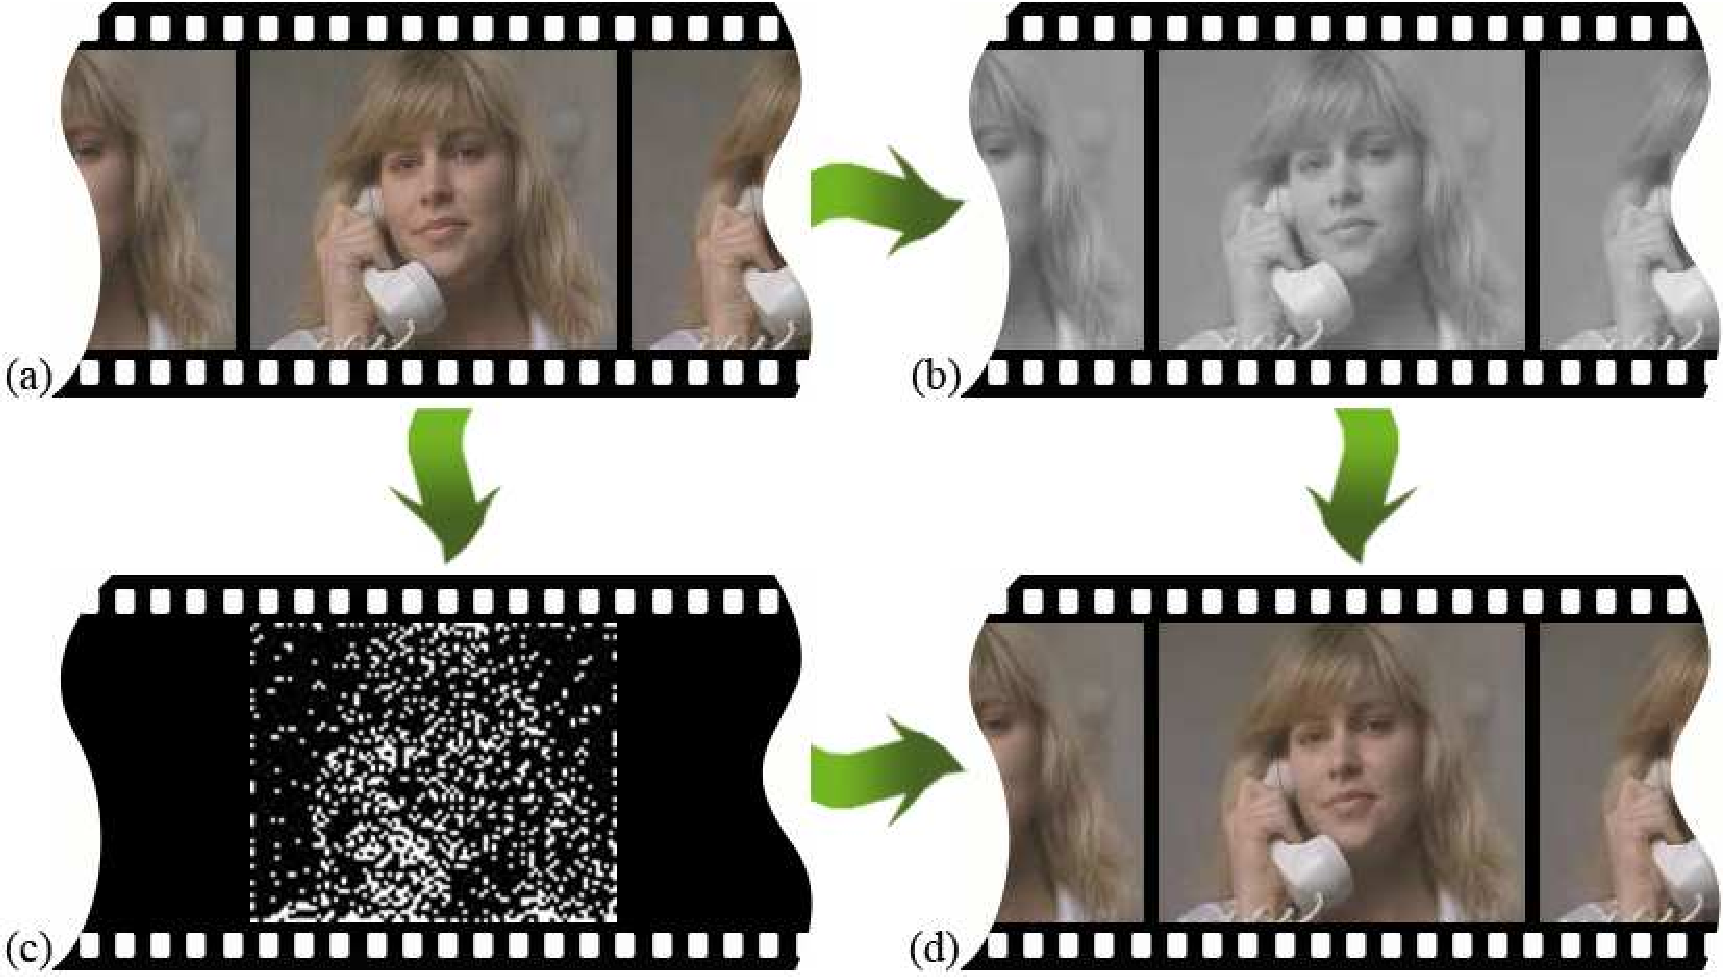
\includegraphics[width=380pt]{images/cycle}}
\caption{\label{fig:cycle}基于学习的视频压缩的例子。 (a) 原始视频帧
(b) 灰度帧 (c) 选取的带有颜色信息的点 (d) 恢复的视频帧}
\end{figure*}

在本文中,我们将从视频压缩这个具体的例子出发,来阐述同时结合时间和空间的正则化
给机器学习问题所带来的性能提升。
视频是一种典型的随着时间轴变化的数据,并且通常在
时间上的变化是比较平滑的,正好是时空正则化的典型应用场景。视频压缩是一项用于缓解
视频存储空间以及传输带宽占用的
关键性技术。视频数据通常包含了许多时间和空间上的冗余信息。相似信息可以通过编码帧内
(空间上的)或帧间(时间上的)差异的方式来进行存储。
典型的压缩方法包括了离散余弦变换、 向量化、分形压缩以及离散小波变换等。

最近 \cite{learning-to-compress-images}
提出了基于机器学习的视频压缩方法。他们提出了和传统的频域转换不同的方式,将原始的带颜色的视频
转化为一个灰度视频,选取一些有代表性的点并存储他们的颜色信息,然后使用灰度视频和带有颜色信息
的点学习出一个统计模型,用于预测其他像素点的颜色值。实验结果表明,在保证图像质量(通过
PSNR
\footnote{http://en.wikipedia.org/wiki/PSNR}进行衡量)的前提下,可以达到不错的压缩效果。

从机器学习的视角来看,这里主要有两个基本的问题。首先是如何选取最有代表性的点,这本质上是一个
主动学习(Active
Learning)的问题。存储灰度视频和选出来的颜色点的信息就是编码的过程。
其次是如何结合选出来的带颜色信息的点和灰度视频来学习一个模型,这在本质上是
一个半监督学习(Semi-supervised
Learning)的问题。用这个模型来恢复原始视频就是解码的过程。在这里有颜色的像素被当作是带标签的
数据,而灰度像素则被当作是无标签的数据。\cite{learning-to-compress-images}
使用了一种非常直接的主动学习的方法:在每一次迭代的时候简单地在预测错误率最高的区域选点。在选
点之后他们使用拉普拉斯正则化的最小二乘法(LapRLS,\cite{Manifold-Regularization-Journal})来
完成半监督学习的问题。他们的方法的最大的不足就是没有任何理论上的依据可以保证使用这种方法选出来
的点可以降低预测的错误率。

在本文中,我们将提出一个针对视频压缩的自主学习和半监督学习的统一框架,并使用时空正则化的方法
对其进行改进以获得性能提升。我们的方法的中心思想是颜色
点的选取和后续的着色过程应该同时进行优化。具体来讲,对于着色的过程,我们假定每个像素的颜色值可以
通过其(时间或空间上的)邻居中灰度值相似的像素的颜色值重新构造出来,并使用正则化的最小二乘法
来学习一个模型;对于选点的过程,我们使用相同的损失函数(loss
function),并使用最小化系数的协方差矩阵的准则来进行选点。然后我们还讨论了如何将自主学习和半监督
学习结合起来应用到视频压缩上面。学习出来的模型不仅用于预测当前的帧,而且还被用于预测后续的相似的
帧,知道 PSNR 分值降低超过了一定的阈值,再重新训练一个模型。图
\ref{fig:cycle} 展示了我们的方法是如何工作的。

论文余下的部分是这样组织的:在第二章中,我们简要地回顾了一下这个领域相关的工作。用于着色的半监督
学习的办法将会在第三章中介绍。第四章介绍如何通过主动学习选取最具代表性的点。然后我们会在第五章中
给出一个用于视频压缩的主动学习和半监督学习的统一框架并运用时空正则化的方法进行改进。实验结果将在
第六章中展示。第七章我们将会进行简要总结并展望后续的工作。


  
\chapter{第二章}

这是第二章,目的是占个位置。你知道《浙大同学爱占坐》这首歌吗?

%==============================================================
%这也是个不需要自己修改的部分。

  \backmatter %结束章节自动编号

  %参考文献
  \addcontentsline{toc}{chapter}{参考文献} % 解决目录中没有相应的参考文献的条目问题
  \chaptermark{参考文献}

%==============================================================

  \bibliography{bibfile/zjubib}

  %附录
  \chapter*{附\quad 录}
\chaptermark{附录}
\addcontentsline{toc}{chapter}{附录} 


  % 这里应该还有个 indices,但我从没见过有使用 indices 的论文,略之。
  %作者简历
  \chapter*{攻读博士学位期间主要研究成果}
\chaptermark{攻读博士学位期间主要研究成果}
\addcontentsline{toc}{chapter}{攻读博士学位期间主要研究成果} 

猪八戒,又名猪刚鬣和天蓬元帅,法号“悟能”,猪脸人身,九齿钉耙为其武器。

猪八戒原是天庭中统领十万天河水兵的天蓬元帅,由于蟠桃会上喝酒醉后调戏月宫仙女嫦娥,打了两千锤后被贬下凡,又投错胎变成猪模样,在高老庄抢占民女。后经观音菩萨指点,拜唐僧为师,一同赴西天取经。取回真经后,猪八戒由于“又有顽心,色情未泯”被封为净坛使者。

后人有鉴于天蓬元帅颇具凡心,善於戏弄逗笑,极具娱乐效果,遂奉为娱乐界、青楼祖师爷。

\begin{itemize}
\item 发表的文章
\item 出版的书籍
\end{itemize}

%==============================================================
%==============================================================
\end{document}
